\begin{frame}{Hetergeneous Multiscale Molecular Dynamics (HMMD)}
\begin{tikzpicture}[scaleall=1.0]
\pcuad{\textwidth}{\textheight}
\path(nw) ++(-1,-0.5) node(graphic1)[anchor=north west]{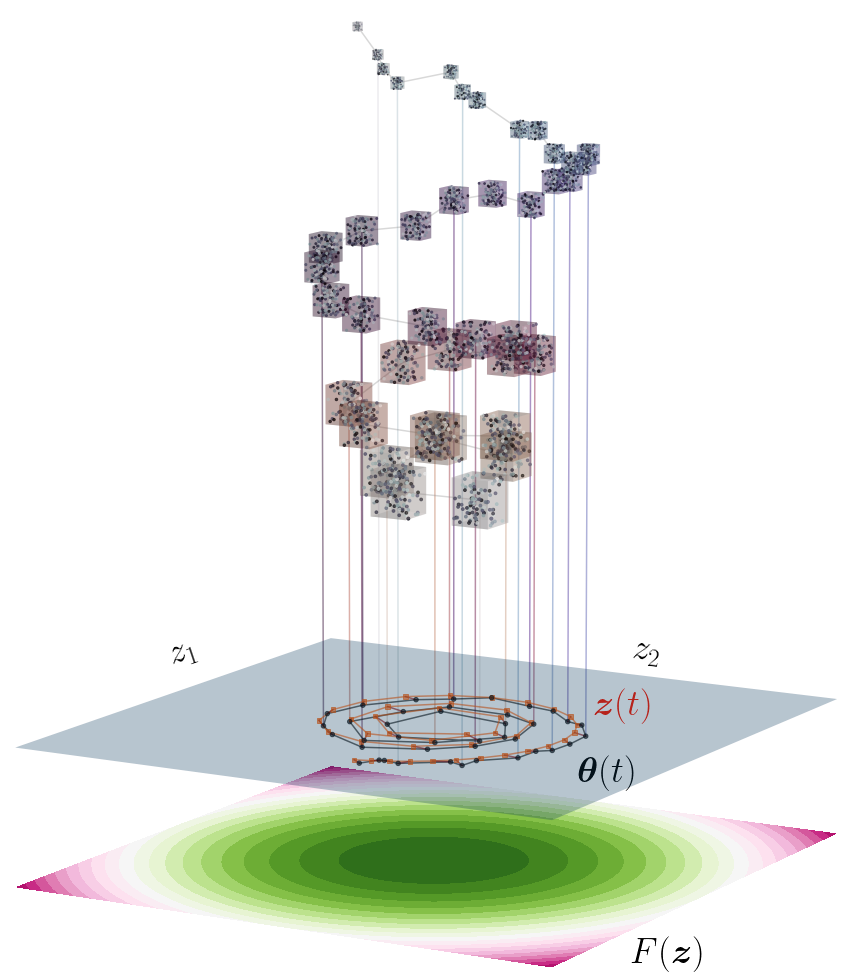
\includegraphics[width=0.6\textwidth]{../hmmdfig2-crop.png}};
\path(np) ++(-1.5,-1) node(line1)[anchor=north west]{Extended configuration space $(\xb^{3N},\ \color{orange!70!black}{\zb^M}\color{black})$}
++(0,-1.5) node(line2)[anchor=west]{$\displaystyle m_i\ddot{x}_i = -\nabla_iV(\xb)-\sum_{j=1}^M\color{green!80!black}{\kappa[\theta_j(\xb)-z_j]}\color{black}\frac{\partial\theta_j}{\partial x_i} + \mbox{e.f.}$}
++(0,-1) node(line3)[anchor=west]{$\displaystyle\bar{m}_j\ddot{z}_j = \sum_{k=1}^{M} \mathcal{M}_{jk}\color{green!80!black}{\kappa[\theta_k(\xb)-z_k]}\color{black} + \color{blue!80!black}{\mbox{bias}}\color{black}$}
++(1,-1.2) node(line4)[anchor=west,align=left] {\textcolor{green!80!black}{Forces} link $\xb$ and $\color{orange!70!black}{\zb}\color{black}$}
++(0,-1) node[anchor=west,align=left,text width=0.6\textwidth] {\textcolor{blue!80!black}{Bias} on $\color{orange!80!black}{\zb}\color{black}$ drives sampling of feature space};
%\draw[] (1.25,2) node {$\thetab(\xb)$};
%\draw[] (2.5,1.75) node {$\zb$};
\end{tikzpicture}
\end{frame}
